\section{Analysis}
	\subsection{Theoretical}
	
	\subsection{Empirical}

		\begin{frame}{Baselines}

		\begin{itemize}
			\item[$\bullet$] balanced quantum k-means (case study)
			\item[$\bullet$] balanced classical k-means (authors implementation)
			\item[$\bullet$] classical k-means scikit-learn implementation
		\end{itemize}

		classical version of the k-means (non balanced) is used since, due to the structure 
		of the dataset, constitute a valid comparison.
		
		\end{frame}

		\begin{frame}{Performance Metrics}
						
			\textbf{Adjusted Rand Index (ARI)}
			\begin{itemize}
				\item[$\bullet$] compare the similarity of two partitions of a dataset
				\item[$\bullet$] range from $-1$ to $1$ (high values indicates the two partitions are similar) 
				\item[$\bullet$] used to compare the target partitions to the partitions produced by clustering 
			\end{itemize}
			
			\textbf{Total Computing time in quantum approach}
			\begin{equation}
				t = t_{QUBO convertion} + t_{embedding} + t_{anealing} + t_{postprocessing}
			\end{equation}
			\begin{itemize}
				\item[$\bullet$] $t_{QUBO convertion}$ time to convert the problem in QUBO
				\item[$\bullet$] $t_{embedding}$ time to embed the QUBO on hardware 	
				\item[$\bullet$] $t_{anealing}$ time to solve the QUBO (anealing time)
				\item[$\bullet$] $t_{postprocessing}$ extract clustering from binary solution
			\end{itemize} 

		\end{frame}

		\begin{frame}{Data Generation}

			synthetic classification datasets created with \textit{make\_classification} (Scikit-learn)	\\
			\textbf{Datasets structure}
			\begin{itemize}
				\item[$\bullet$] \textbf{N} points	
				\item[$\bullet$] \textbf{k} classes	
				\item[$\bullet$] \textbf{1} cluster per class	
				\item[$\bullet$] \textbf{d} features 
				\item[$\bullet$] clusters centered on a \textit{d}-dimensional hypercube (with side length $2.0$)  
				\item[$\bullet$] points generated from a normal dist. about their cluster center (std $1.0$)   
				\item[$\bullet$] each class made of $\frac{N}{k}$ points   
			\end{itemize}
			
		\end{frame}

		\begin{frame}{Hardware Configuration}	
			\textbf{Classical Machine}
			\begin{itemize}
				\item[$\bullet$] 2.7 GHz Dual-Core Intel i5 
				\item[$\bullet$] 8 GB 1.867 MHz DDR3 memory 
			\end{itemize}

			\textbf{Quantum Machine}
			\begin{itemize}
				\item[$\bullet$] D-Wave 2000Q quantum computer 
				\item[$\bullet$] 2048 qubits, 5600 inter-qubit connections
			\end{itemize}

			\textbf{Technical Aspects}
			\begin{itemize}
				\item[$\bullet$] quantum approach pre/post-processing done via the above classical machine
				\item[$\bullet$] quantum anealing operation perfomed 100 times for each experiment   
				\item[$\bullet$] only ground state is used % TODO: find out the meaning  
			\end{itemize}			
					
		\end{frame}
	
	\subsection{Benchmark}
	\begin{frame}[allowframebreaks]{Clustering a Benchmark Data Set}
		\textbf{The Iris Dataset}
		\begin{itemize}
			\item[$\bullet$] Reduced due to qubit limitations on modern hardware
			\item[$\bullet$] Pick $N/k$ points from $2\leq k \leq3$ of the data set's classes
		\end{itemize}
	
		\textbf{Experiments Run}
		\begin{itemize}
			\item[$\bullet$] All the 3 clustering algorithms were tested
			\item[$\bullet$] Experiments are run on 50 subsets of the dataset
		\end{itemize}
	
		\textbf{Results}
		\begin{itemize}
			\item[$\bullet$] $k=2$
			\begin{itemize}
				\item[$\circ$] Trivial case, points are linearly separable
				\item[$\circ$] Classical algorithms perform better than quantum
				\item[$\circ$] Evident as the number of binary variables $(Nk)$ increases
			\end{itemize}
			\framebreak
			\item[$\bullet$] $k=3$
			\begin{itemize}
				\item[$\circ$] time to extract rforms \textbf{Scikit-Learn} implementation
				\item[$\circ$] Performance of the QA degrades as the problem size increases
			\end{itemize}
		\end{itemize}
		\begin{center}
			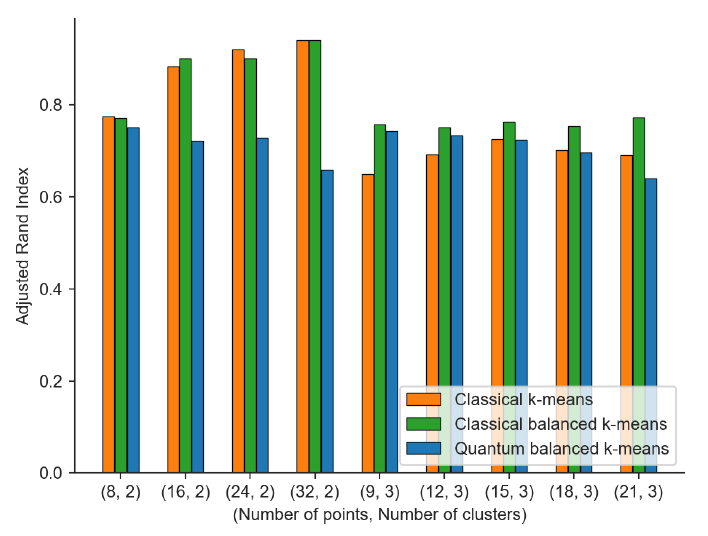
\includegraphics[scale=0.45]{Iris_ARI_table.png}
		\end{center}
	\end{frame}